% Drawing 144/03-6 -- folder 144, batch 03, archive page 56 (PDF page 57).
% Transcription: Un arbre trivalent dont les sommets portent les types $0$ et $1$ ; à droite une arête repliée qui aboutit en un sommet de type $\infty$, avec les deux repères $r$ et $r'$ de part et d'autre (sens de rotation opposés) dans un contour fin ; en bas une région hachurée autour d'un sommet $\infty$ où figurent $\sigma_{\infty}r_{1}$, $\sigma_{0}r_{1}$, $\sigma_{1}r_{1}$ et $r_{1}$.
% Kind: trivalent tree with vertex types, folded edge, frames. Method 2 (schematic redraw from the facsimile). Status: partial.
% Notes: Tree with vertices of type 0 and midpoints 1; on the right the folded edge ends in a vertex of type infinity, with the frames r and r' (opposite senses of rotation) inside a thin contour. Bottom: the hatched region round a vertex, overinked; its labels sigma_infty r_1, sigma_0 r_1, sigma_1 r_1, r_1 are placed as read but are partly illegible under the hatching.
% Coordinates: 1 unit = 1 mm = 1/100 of the crop width (bbox in page fractions: [0.25, 0.05, 0.65, 0.245]).
% Redrawn by Claude (claude-opus-5-5), issue #73, 2026-11-07; not checked by a human; not compiled (no TeX in the session).
% Rights: reproduces part of the work -- behind RENDER_TRANSCRIPTS, never published by itself.
\documentclass[tikz,border=3pt]{standalone}
\usepackage{amsmath,amssymb}
\usetikzlibrary{patterns,arrows.meta}
\tikzset{pencil/.style={black!45}, struck/.style={black!35}, mark/.style={circle,draw,inner sep=1.3pt}, pt/.style={circle,fill,inner sep=0.9pt}, opt/.style={circle,draw,fill=white,inner sep=1.1pt}}
\begin{document}
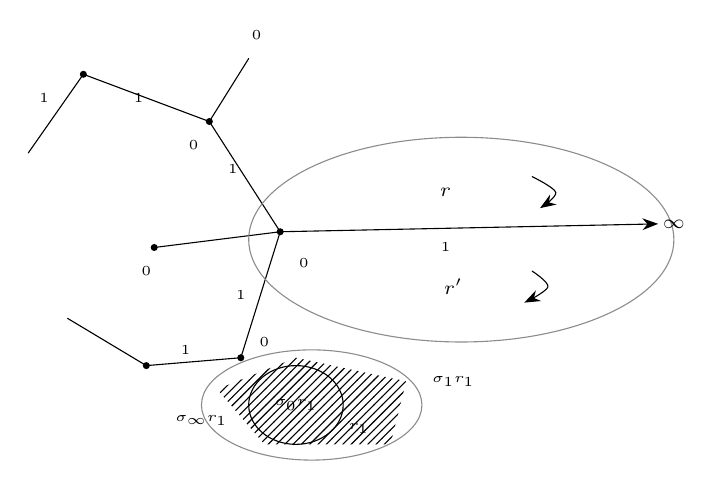
\begin{tikzpicture}[x=1mm,y=1mm,line cap=round,line join=round,font=\scriptsize]
\draw (6,-26) -- (13,-16) -- (29,-22) -- (34,-14);
\draw (29,-22) -- (38,-36) -- (22,-38);
\draw[-{Stealth[length=2mm]}] (38,-36) -- (86,-35);
\draw (38,-36) -- (33,-52) -- (21,-53) -- (11,-47);
\node[pt] at (13,-16) {};
\node[pt] at (29,-22) {};
\node[pt] at (38,-36) {};
\node[pt] at (22,-38) {};
\node[pt] at (33,-52) {};
\node[pt] at (21,-53) {};
\draw[pencil] (61,-37) ellipse[x radius=27, y radius=13];
\node[inner sep=1pt] at (27,-25) {\tiny $0$};
\node[inner sep=1pt] at (35,-11) {\tiny $0$};
\node[inner sep=1pt] at (21,-41) {\tiny $0$};
\node[inner sep=1pt] at (41,-40) {\tiny $0$};
\node[inner sep=1pt] at (36,-50) {\tiny $0$};
\node[inner sep=1pt] at (8,-19) {\tiny $1$};
\node[inner sep=1pt] at (20,-19) {\tiny $1$};
\node[inner sep=1pt] at (32,-28) {\tiny $1$};
\node[inner sep=1pt] at (33,-44) {\tiny $1$};
\node[inner sep=1pt] at (26,-51) {\tiny $1$};
\node[inner sep=1pt] at (59,-38) {\tiny $1$};
\node[inner sep=1pt] at (88,-35) {\scriptsize $\infty$};
\node[inner sep=1pt] at (59,-31) {\scriptsize $r$};
\node[inner sep=1pt] at (60,-43) {\scriptsize $r'$};
\draw[-{Stealth[length=2mm]}] plot[smooth, tension=0.55] coordinates {(70,-29) (73,-31) (71,-33)};
\draw[-{Stealth[length=2mm]}] plot[smooth, tension=0.55] coordinates {(70,-41) (72,-43) (69,-45)};
\draw[pencil] (42,-58) ellipse[x radius=14, y radius=7];
\fill[pattern=north east lines] (30,-56) -- (40,-52) -- (54,-55) -- (52,-63) -- (36,-63) -- cycle;
\draw (40,-58) ellipse[x radius=6, y radius=5];
\node[inner sep=1pt] at (28,-60) {\tiny $\sigma_\infty r_1$};
\node[inner sep=1pt] at (40,-58) {\tiny $\sigma_0 r_1$};
\node[inner sep=1pt] at (60,-55) {\tiny $\sigma_1 r_1$};
\node[inner sep=1pt] at (48,-61) {\tiny $r_1$};
\end{tikzpicture}
\end{document}
